\documentclass[12pt]{article}
\usepackage[czech]{babel}
\usepackage[utf8]{inputenc}
\usepackage[plainpages=false,pdfpagelabels,unicode]{hyperref}
\usepackage[pdftex]{graphicx}
\usepackage[margin=3cm, includefoot]{geometry}

\begin{document}

\title{Protokol z předmětu Atomová a molekulová spektroskopie}
\author{Vlasta Štěpánová a Pavel Ondračka}
\date{20.10.2011}
\maketitle

\section{Úvod}
Cílem tohoto praktika bylo seznámit se s principy atomové a molekulové spektroskopie a zjistit jak vypadají spektra nejběžnějších plynů a světelných zdrojů. Dalším účelem praktika bylo seznámit se s obsluhou spektrometru a metodami vyhodnocování naměřených dat. Během praktika byla měřena celá škála světelných zdrojů: žárovka, doutnavka, LED, zářivka, výbojové trubice (s vodíkem, dusíkem) a rtuťová lampa.

\subsection{HORIBA JOBIN-YVON FHR 1000}
FHR 1000 je automatizovaný spektrometr od firmy HORIBA Jobin-Yvon
s konfigurací Czerny-Turner umožňující snímání s vysokou přesností v oblasti vlnových délek od UV po IR v závislosti na použité mřížce a
detektoru.
Základní části spektrometru FHR 1000 jsou: vstupní štěrbina, dvě konkávní
zrcadla, rovinná difrakční mřížka a detektory.
Světlo je ze zdroje přiváděno na vstup spektrometru pomocí optického vlákna
a je promítáno pomocí zrcadel na vstupní štěrbinu, jejíž šířku můžeme nastavit 
elektronicky v rozmezí 0--2\,mm s krokem 2\,$\mu$m, a výšku můžeme omezit
manuálně. Ze štěrbiny dopadá světlo na
první konkávní zrcadlo, které z něj vytváří rovnoběžný svazek. Ten dopadá
na rovinnou difrakční mřížku, která se může otáčet kolem své osy a její pohyb
je řízen rovněž elektronicky. Natáčením mřížky vybíráme oblast vlnových
délek, které dopadají na druhé zrcadlo a to je promítá na detektor. Ohnisková vzdálenost je 1\,m. Hustota vrypů použité mřížky byla 2400 vrypů na mm$^2$, případně 3600 vrypů na mm$^2$. Jako detektor byla použita CCD kamera o rozlišení 2048$\times$512\,pixelů chlazená čtyřstupňovým peltierovým článkem. 
 
\section{Měření}

\subsection{Závislost intenzity čáry na integrační době}
Prvním ukolem tohoto praktika bylo změřit jak závisí intenzita spektrální čáry na integrační době. Pro deset integračních časů v rozmezí 0,1--1\,s byla měřena intenzita čáry rtuti na 431\,nm. Výsledná intenzita v grafu je rozdíl absolutní intenzity a intenzity pozadí.Výsledky měření jsou na obrázku \ref{fig:ukol1}. Ukázalo se, že závislost je lineární.

\begin{figure}[h!]
  \centering
  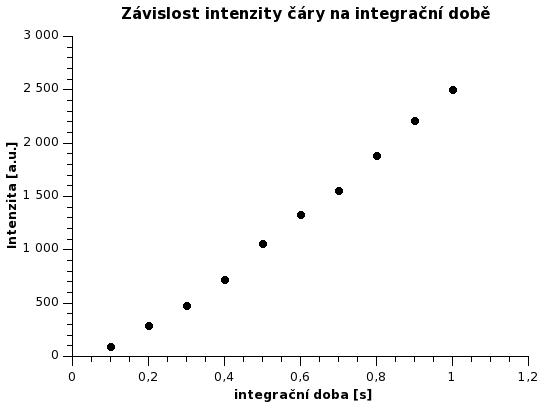
\includegraphics[width=13cm]{img/Graph1.png}
  \caption{Závislost intenzity čáry na integrační době}
  \label{fig:ukol1} 
\end{figure}


\subsection{Spektrální rtuťová lampa}
Byla měřena jednak celá oblast od 250\,nm do 650\,nm (obrázek \ref{fig:rtut}), pak také detail v oblasti 300--450\,nm (obrázek \ref{fig:rtut2}). Čáry rtuti jsou popsány v tabulce \ref{fig:Hg}

\begin{figure}[h!]
  \centering
  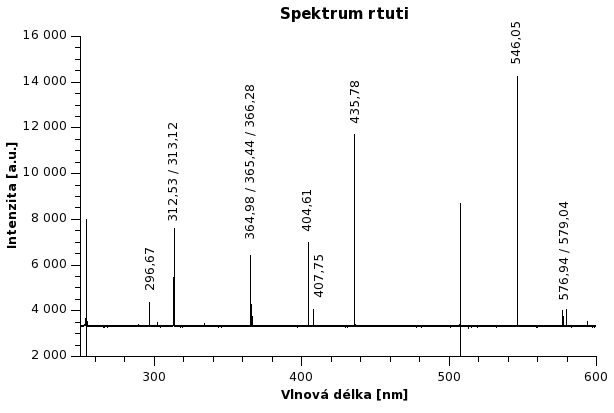
\includegraphics[width=13cm]{img/rtut.png}
  \caption{Spektrum rtuťové lampy}
  \label{fig:rtut} 
\end{figure}

\begin{figure}[h!]
  \centering
  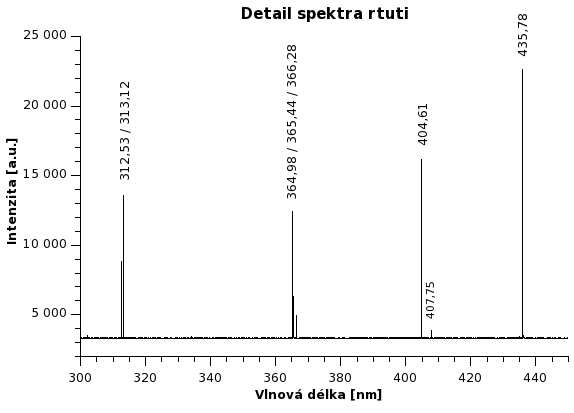
\includegraphics[width=13cm]{img/rtut2.png}
  \caption{Detail spektra rtuťové lampy}
  \label{fig:rtut2} 
\end{figure}

\begin{table}[h!]
 \centering
 \begin{tabular}{|c|c|c|c|c|}
  \hline
  {\bf } & {\bf měřená $\lambda$} & {\bf tabelovaná $\lambda$} & {\bf konfigurace} & {\bf termy} \\
	 & {\bf[nm]} & {\bf[nm]} & & \\   
   \hline \hline
	Hg I & 296,67 & 296,72 & $5d^{10}6s6p - 5d^{10}6s6d$ & $^3P^*-{^3D}  $ \\
	Hg I & 312,53 & 312,56 & $5d^{10}6s6p - 5d^{10}6s6d$ & $^3P^*-{^3D}  $ \\
	Hg I & 313,12 & 313,15 & $5d^{10}6s6p - 5d^{10}6s6d$ & $^3P^*-{^3D}  $ \\

	Hg I & 364,98 & 365,01 & $5d^{10}6s6p - 5d^{10}6s6d$ & $^3P^*-{^3D}  $ \\
	Hg I & 365,44 & 365,48 & $5d^{10}6s6p - 5d^{10}6s6d$ & $^3P^*-{^3D} $ \\
	Hg I & 366,28 & 366,32 & $5d^{10}6s6p - 5d^{10}6s6d$ & $^3P^*-{^3D} $ \\

	Hg I & 404,61 & 404,65 & $5d^{10}6s6p - 5d^{10}6s7s$ & $^3P^*-{^3S}  $ \\
	Hg I & 407,75 & 407,78 & $5d^{10}6s6p - 5d^{10}6s7s$ & $^3P^*-{^1S}  $ \\
	Hg I & 435,78 & 435,83 & $5d^{10}6s6p - 5d^{10}6s7s$ & $^3P^*-{^3S}  $ \\

	Hg I & 546,05 & 546,07 & $5d^{10}6s6p - 5d^{10}6s7s$ & $^3P^*-{^3S}  $ \\

	Hg I & 576,94 & 576,96 & $5d^{10}6s6p - 5d^{10}6s6d$ & $^1P^*-{^3D} $ \\
	Hg I & 579,04 & 579,07 & $5d^{10}6s6p - 5d^{10}6s6d$ & $^1P^*-{^1D} $ \\
  \hline
  \end{tabular}
  \caption{Některé píky rtuti}
  \label{fig:Hg}
\end{table}

\clearpage

\subsection{Žárovka}
Během tohoto úkolu bylo měřeno spektrum obyčejné žárovky a také byla vyzkoušena funkce světelných filtrů. Na obrázku \ref{fig:zarovka} můžeme vidět, že záření žárovky odpovídá záření černého tělesa. Z Wienova posunovacího zákona můžeme odhadnout teplotu vlákna. Pro maximální intenzitu na 664\,nm to odpovídá teplotě asi 4360\,K. Bohužel je vidět, že tato teplota je vysoko nad bodem tání wolframu, z nějakého důvodu tedy Wienův posunovací zákon nelze na žárovku aplikovat. Také se podařilo potvrdit funkci filtru, je vidět že z celého spektra po použití filtru naměříme nenulovou intenzitu jen v okolí 635\,nm. To odpovídá tmavě červené barvě, což se shoduje s vizuální barvou filtru.

\begin{figure}[h!]
  \centering
  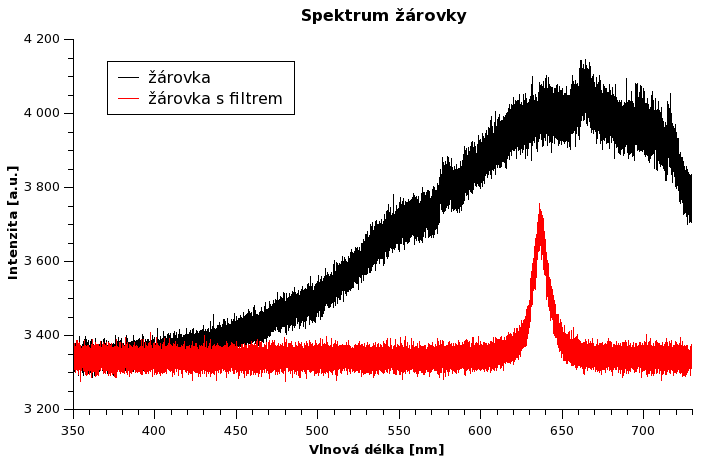
\includegraphics[width=13cm]{img/zarovka.png}
  \caption{Spektrum žárovky}
  \label{fig:zarovka} 
\end{figure}

\subsection{Zářivka}
Základem zářivky je výbojová trubice naplněná rtuťovými parami. Rtuť září převážně v UV oblasti, proto je povrch trubice pokryt luminoforem, který absorbuje UV světlo a září ve viditelné oblasti. Proto můžeme ve spektru zářivky (obrázek \ref{fig:zarivka}) vidět jak čarové spektrum rtuti, tak spojité spektrum luminoforu. Největší píky rtuti jsou opět bohužel deformované kvůli problémům se spektrometrem, proto byly určeny některé menší. Široké píky pravděpodobně všechny náleží luminoforu.

\begin{figure}[h!]
  \centering
  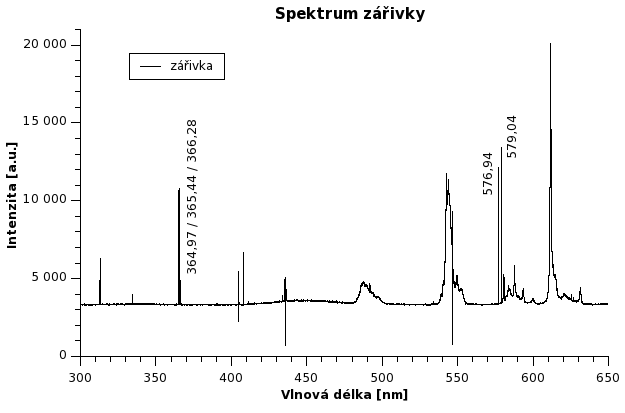
\includegraphics[width=13cm]{img/zarivka.png}
  \caption{Spektrum zářivky, popis něterých identifikovaných píků je v tabulce \ref{fig:Hg}}
  \label{fig:zarivka} 
\end{figure}


\subsection{Doutnavka}
Doutnavka je nízkotlaká plynem plněná výbojka se studenou katodou pracující v oblasti samostatného doutnavého výboje. Odtud pochází její název. Bývá většinou plněna neonem, někdy s příměsí argonu. Na obrázku \ref{fig:doutnavka} je naměřené spektrum doutnavky. Ukázalo se že je opravdu plněna neonem, bez jiných příměsí.

\begin{figure}[h!]
  \centering
  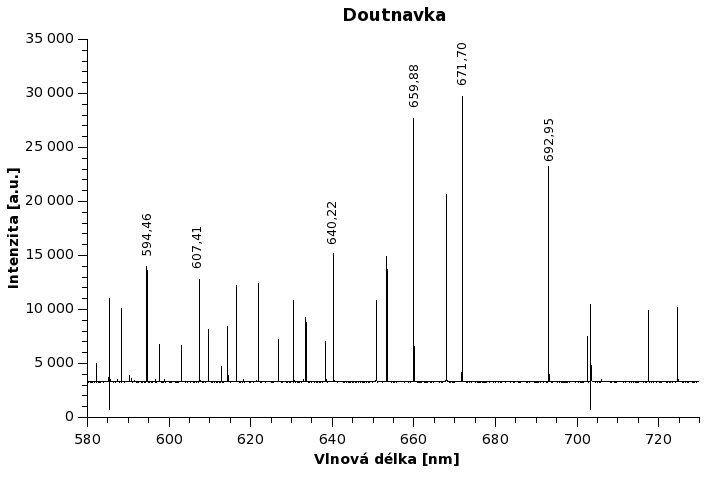
\includegraphics[width=13cm]{img/doutnavka.png}
  \caption{Spektrum doutnavky, popis identifikovaných píků je v tabulce \ref{ref:Ne}}
  \label{fig:doutnavka} 
\end{figure}

\begin{table}[h!]
 \centering
 \begin{tabular}{|c|c|c|c|c|}
  \hline
  {\bf } & {\bf měřená $\lambda$} & {\bf tabelovaná $\lambda$} & {\bf konfigurace} & {\bf termy} \\
	 & {\bf[nm]} & {\bf[nm]} & & \\   
   \hline \hline
	Ne I & 594,46 & 594,48 & $2s^22p^5(^2P^*_{3/2})3s - 2s^22p^5(^2P^*_{1/2})3p$ & $^2[3/2]^*-{^2[3/2]} $ \\
	Ne I & 607,41 & 607,43 & $2s^22p^5(^2P^*_{3/2})3s - 2s^22p^5(^2P^*_{3/2})3p$ & $^2[3/2]^*-{^2[1/2]} $ \\
	Ne I & 640,22 & 640,22 & $2s^22p^5(^2P^*_{3/2})3p - 2s^22p^5(^2P^*_{3/2})3p$ & $^2[3/2]^*-{^2[5/2]} $ \\
	Ne I & 659,88 & 659,90 & $2s^22p^5(^2P^*_{1/2})3s - 2s^22p^5(^2P^*_{1/2})3p$ & $^2[1/2]^*-{^2[1/2]} $ \\

	Ne I & 671,70 & 671,70 & $2s^22p^5(^2P^*_{1/2})3s - 2s^22p^5(^2P^*_{1/2})3p$ & $^2[1/2]^*-{^2[3/2]} $ \\
	Ne I & 692,95 & 692,94 & $2s^22p^5(^2P^*_{1/2})3s - 2s^22p^5(^2P^*_{3/2})3p$ & $^2[1/2]^*-{^2[3/2]} $ \\
   \hline
  \end{tabular}
  \caption{Některé identifikované píky ve spektru doutnavky}
  \label{ref:Ne}
\end{table}
\clearpage


\subsection{LED}
Pro LED je typické nekoherentní světlo s úzkým spektrem. Barva LED závisí na vlastnostech použitého polovodiče a příměsích. Vlnová délka se může pohybovat od IR až po UV oblast. Naměřené spektra jsou na obrázku \ref{fig:dioda}.

Bílého světla můžeme dosáhnout dvěma efekty. Buď kombinací tří LED (červené, zelené a modré), případně jen jednou barvou a použitím luminoforu. Podle průběhu spektra je pravděpodobné, že se jedná o druhou možnost. Pík na 460\,nm je modrá dioda (pravděpodobně GaN), záření od 500\,nm do 700\,nm připadá luminoforu. Běžný žlutý luminofor je například yttrito-hlinitý granát s dopovaným Cerem (Ce$^{3+}$:YAG), ten má emisní maximum přibližně 550\,nm, to odpovídá naměřenému spektru.

\begin{figure}[h!]
  \centering
  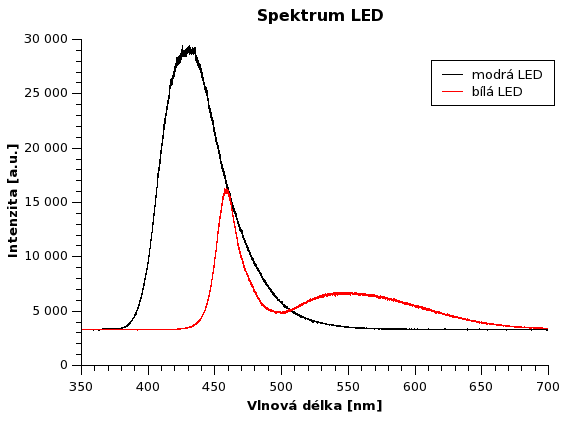
\includegraphics[width=13cm]{img/diody.png}
  \caption{Spektrum LED}
  \label{fig:dioda} 
\end{figure}
\clearpage

\subsection{Geislerova trubice}
\subsubsection{Geislerova trubice s dusíkem}
První Geislerova trubice byla plněna dusíkem. Spektrum je zobrazeno na obrázku \ref{fig:dusik}. Že se jedná o molekulový plyn je jasně patrné z vibračních pásů, které nebyly přítomné v žádném z dosud měřených (atomových plynů). 

\begin{figure}[h!]
  \centering
  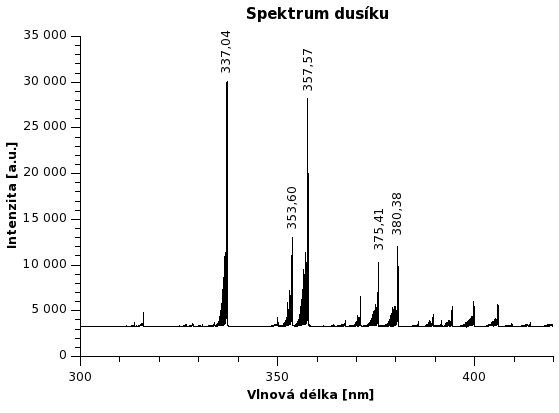
\includegraphics[width=13cm]{img/n2.png}
  \caption{Spektrum molekulárního dusíku, popis identifikovaných píků je v tabulce \ref{ref:n2}}
  \label{fig:dusik} 
\end{figure}

\begin{table}[h!]
 \centering
 \begin{tabular}{|c|c|c|c|c|}
  \hline
  {\bf } & {\bf měřená $\lambda$ [nm]} & {\bf tabelovaná $\lambda$ [nm]} \\
   \hline \hline
	N$_2$ 0--0 & 337,04 & 337,13 \\
	N$_2$ 1--2 & 353,60 & 353,67 \\
	N$_2$ 0--1 & 357,57 & 357,69 \\
	N$_2$ 1--3 & 375,41 & 375,54 \\
	N$_2$ 0--2 & 380,38 & 380,49 \\
   \hline
  \end{tabular}
  \caption{Některé identifikované píky ve spektru dusíku}
  \label{ref:n2}
\end{table}

\subsubsection{Geislerova trubice s vodíkem}
Dalším další geislerova trubice byla plněna vodíkem. Na obrázku \ref{fig:h} jsou vidět jednak výrazné píky H I třeba na 486,10\,nm a 656,28\,nm a také oblasti píků H$_2$ (570--630\,nm).

\begin{figure}[h!]
  \centering
  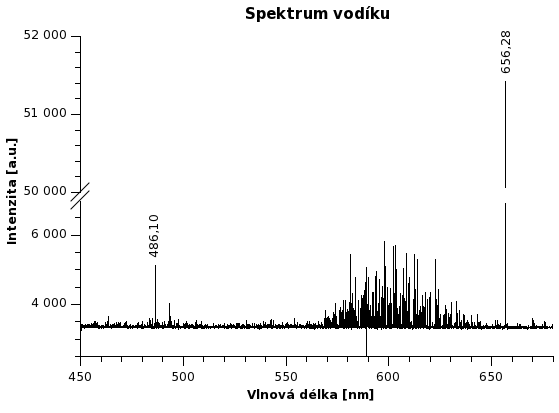
\includegraphics[width=13cm]{img/h.png}
  \caption{Spektrum vodíku}
  \label{fig:h} 
\end{figure}
\clearpage


\subsection{Určení neznámého plynu}
Posledním úkolem praktika bylo pomocí spektroskopie určit druh plynu ve výbojové trubici. Jelikož je z obrázku \ref{fig:argon} jasně patrné, že se jedná o atomový plyn (nejsou viditelné žádné vibrační píky), zúžil se výběr v podstatě jen na vzácné plyny. Podle polohy píků se ukázalo, že plyn v trubici je argon. 

\begin{figure}[h!]
  \centering
  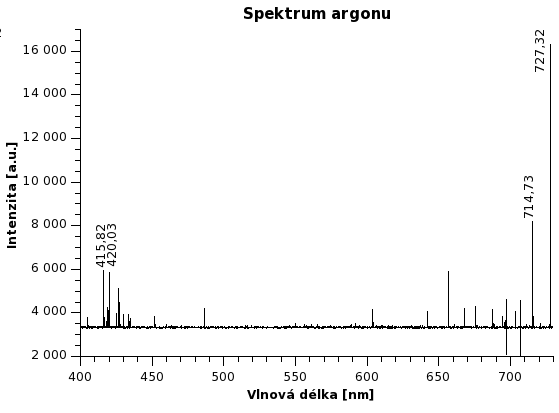
\includegraphics[width=13cm]{img/argon.png}
  \caption{Spektrum argonu, popis identifikovaných píků je v tabulce \ref{ref:Ar}}
  \label{fig:argon} 
\end{figure}

\begin{table}[h!]
 \centering
 \begin{tabular}{|c|c|c|c|c|}
  \hline
  {\bf } & {\bf měřená $\lambda$} & {\bf tabelovaná $\lambda$} & {\bf konfigurace} & {\bf termy} \\
	 & {\bf[nm]} & {\bf[nm]} & & \\   
   \hline \hline
	Ar I & 415,82 & 415,86 & $3s^23p^5(^2P^*_{3/2})4s - 3s^23p^5(^2P^*_{3/2})5p$ & $^2[3/2]^*-{^2[3/2]} $ \\
	Ar I & 420,03 & 420,07 & $3s^23p^5(^2P^*_{3/2})4s - 3s^23p^5(^2P^*_{3/2})5p$ & $^2[3/2]^*-{^2[5/2]} $ \\
	Ar I & 714,73 & 714,70 & $3s^23p^5(^2P^*_{3/2})4s - 3s^23p^5(^2P^*_{1/2})4p$ & $^2[3/2]^*-{^2[3/2]} $ \\
	Ar I & 727,32 & 727,29 & $3s^23p^5(^2P^*_{3/2})4s - 3s^23p^5(^2P^*_{1/2})4p$ & $^2[3/2]^*-{^2[1/2]} $ \\
   \hline
  \end{tabular}
  \caption{Některé identifikované píky ve spektru argonu}
  \label{ref:Ar}
\end{table}

\section{Závěr}
Měření bylo úspěšně. Ukázalo se, že intenzita spektrální čáry je přímo úměrná integrační době. Všechna naměřené spektra mají očekávaný tvar. Většina spekter obsahuje pouze měřené plyny, vliv externího rušení se podařilo omezit na minimum (například tím že bylo po celou dobu zhasnuto). Spektrum žárovky odpovídá přibližně spektru černého tělesa. Spektra doutnavky, zářivky a LED také splňují teoretická očekávání. Ve spektru molekulových plynů můžeme pozorovat intenzivní vibrační pásy. Také se podařilo úspěšně identifikovat neznámý plyn. Jednalo se o argon. Bohužel při měření byla nějaká závada na spektrometru, proto jsou některé píky zobrazeny do záporných hodnot. Jedná se povětšinou o nejintenzivnější píky daného vzorku. Tyto píky nebyly pro identifikaci používány, což poněkud celou práci ztížilo.
\end{document}
